\section{Theoretical Analysis}
\label{sec:analysis}

\subsection{Question 1: Node Analysis}
This preliminary analysis of the circuit is the basis of the rest of the work and to do this we used the nodal method in the same way as used in T1. We have the equations: (the nomenclature for all nodes and branches is present in figure 1).\par
\emph{Node 0 (ground):}
\begin{equation}
    \frac{1}{R_1}(V_2-V_1) + \frac{1}{R_4}(V_5-0)- I_d  = 0
\end{equation}\par

\emph{Node 2:}
\begin{equation}
    \frac{1}{R_1}(V_1-V_2) + \frac{1}{R_2}(V_3-V_2) + \frac{1}{R_3}(V_5-V_2) = 0
\end{equation}\par

\emph{Node 3:}
\begin{equation}
    \frac{1}{R_2}(V_2-V_3) + I_b  = 0
\end{equation}\par

\emph{Node 5:}
\begin{equation}
    \frac{1}{R_3}(V_2-V_5) + \frac{1}{R_5}(V_6-V_5) + \frac{1}{R_4}(0-V_5) - I_d = 0
\end{equation}\par

\emph{Node 6:}
\begin{equation}
    \frac{1}{R_5}(V_5-V_6) - I_b - I_c = 0
\end{equation}\par

\emph{Node 7:}
\begin{equation}
    \frac{1}{R_6}(V_7-0) + I_d  = 0
\end{equation}\par

\emph{Node 8:}
\begin{equation}
    \frac{1}{R_7}(V_7-V_8) - I_d + I_c = 0
\end{equation}\par

\emph{Additional equation:}
\begin{equation}
     V_5 - V_8 - K_dI_d = 0
\end{equation}\par

\emph{Additional equation:}
\begin{equation}
     V_2 - V_5 - \frac{I_b}{K_b} = 0
\end{equation}\par

And the results are shown in the following table:

\begin{center}
  \begin{tabular}{ | c | c | }
    \hline    
    {\bf Name} & {\bf Value [A or V]} \\ \hline
    $V_1$ & 5.025226e+00 \\ \hline 
$V_2$ & 4.724476e+00 \\ \hline 
$V_3$ & 4.104661e+00 \\ \hline 
$V_5$ & 4.765766e+00 \\ \hline 
$V_6$ & 5.702373e+00 \\ \hline 
$V_7$ & -1.847813e+00 \\ \hline 
$V_8$ & -2.790649e+00 \\ \hline 
$I_1$ & -2.870701e-04 \\ \hline 
$I_2$ & -3.006765e-04 \\ \hline 
$I_3$ & 1.360640e-05 \\ \hline 
$I_4$ & 1.190255e-03 \\ \hline 
$I_5$ & 3.006765e-04 \\ \hline 
$I_6$ & 9.031846e-04 \\ \hline 
$I_7$ & 9.031846e-04 \\ \hline 
$I_s$ & -2.870701e-04 \\ \hline 
$I_d$ & 9.031846e-04 \\ \hline 
$I_b$ & -3.006765e-04 \\ \hline 
$I_c$ & -2.168404e-19 \\ 

    \hline
  \end{tabular}
\end{center}
All the variables preceded by I are currents and are expressed in Ampere, the other variables, preceeded by V are voltages and are expressed in Volt.



\subsection{Question 2: Equivalent Resistance ($R_{e_q}$)}
The resolution of this question was based on the suggestion presented. Firstly, we set $V_s =0$ and replaced the capacitor by a voltage source $V_x = V_6 - V_8$ and ran the nodal analysis in order to obtain the current $I_x$ witch is the current supplied by $V_x$.\par
Then, with the equation: 
\begin{equation}
     R_{e_q} = \frac{V_x}{I_x}
\end{equation}\par
We obtain the Equivalent resistance. \par 
The time constant $\tau$ is calculated by doing $\tau=R_{e_q}C$\par
Basically, the procedure was based on \emph{Thévenin} theorem. Since, the capacitor was replaced by a Voltage source witch terminals have the same difference of potential as $V_6 - V_8$ in Question 1, this is a known variable and $I_x$ can also be obtainned by running the nodal method with $V_s = 0$. We needed to do this because there is no easiest way to calculate the Equivalent Resistance in a circuit where there are resistances in paralell, series and a capacitor.

The results:

\begin{center}
  \begin{tabular}{ | c | c | }
    \hline    
    {\bf Name} & {\bf Value [A or V]} \\ \hline
    $V_x$ & 8.493021e+00 \\ \hline 
$V_1$ & 0.000000e+00 \\ \hline 
$V_2$ & 0.000000e+00 \\ \hline 
$V_3$ & -0.000000e+00 \\ \hline 
$V_5$ & 0.000000e+00 \\ \hline 
$V_6$ & 8.493021e+00 \\ \hline 
$V_7$ & 0.000000e+00 \\ \hline 
$V_8$ & 0.000000e+00 \\ \hline 
$I_1$ & 0.000000e+00 \\ \hline 
$I_2$ & 0.000000e+00 \\ \hline 
$I_3$ & 0.000000e+00 \\ \hline 
$I_4$ & 0.000000e+00 \\ \hline 
$I_5$ & 2.726493e-03 \\ \hline 
$I_6$ & -0.000000e+00 \\ \hline 
$I_7$ & -0.000000e+00 \\ \hline 
$I_s$ & 0.000000e+00 \\ \hline 
$I_d$ & -0.000000e+00 \\ \hline 
$I_b$ & 0.000000e+00 \\ \hline 
$I_x$ & 2.726493e-03 \\ \hline 
$Req (kOhm)$ & 3.114999e+00 \\ \hline 
$tau (ms)$ & 3.145605e+00 \\ 

    \hline
  \end{tabular}
\end{center}


\subsection{Question 3: Natural solution $v_{6_t}(t)$}
The natural solution $v_{6_t}(t)$ in the interval [0,20]ms calculating:
\begin{equation}
     v_{6_n} = {V_x-V_8}e^{\frac{-t}{\tau}}
\end{equation}\par
Where $V_x$ is the same as in question 1 ($t<0$).
By doing this, the plot obtained is the one shown below:

\begin{figure}[H] \centering
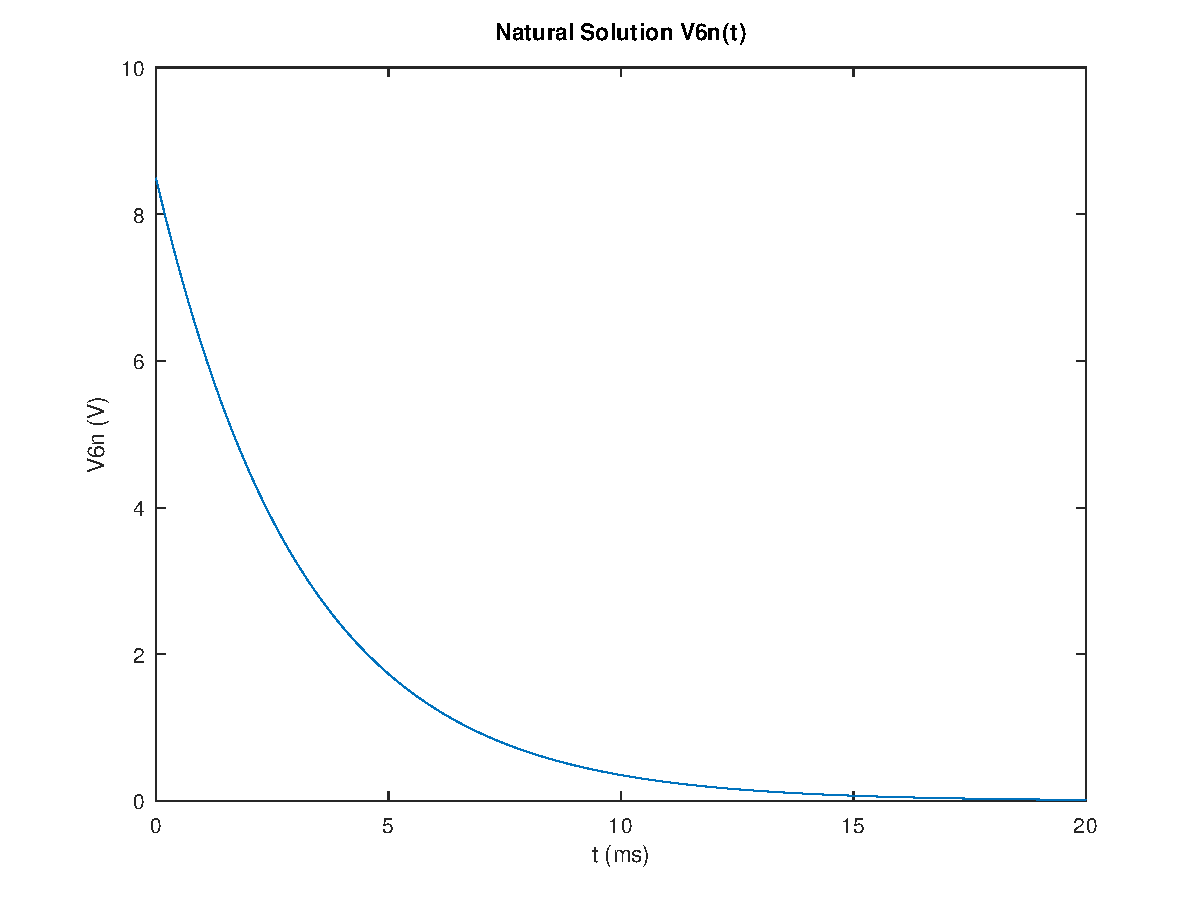
\includegraphics[width=0.7\linewidth]{../mat/alinea3.pdf}
\caption{Plot alinea 3.}
\label{fig:plot3}
\end{figure}


\subsection{Question 4: Forced solution $v_{6_t}(t)$ (f=1Khz)}
In this question, we have used a phasor voltage source $V_s = 1$, so:
\begin{equation}
     v_s = {V_s}e^{-i\frac{\pi}{2}}
\end{equation}\par
Then, replacing C with  impedance $Z_c$ and running the nodal analysis to determine the phasor voltages in all nodes we have the following results:\par

\begin{center}
  \begin{tabular}{ | c | c | }
    \hline    
    {\bf Name} & {\bf Value [A or V]} \\ \hline
    $V_1$ & -0.000000e+00 \\ \hline 
$V_2$ & 3.924207e-19 \\ \hline 
$V_3$ & 6.411465e-19 \\ \hline 
$V_5$ & 3.758515e-19 \\ \hline 
$V_6$ & -8.529278e-02 \\ \hline 
$V_7$ & -9.190910e-20 \\ \hline 
$V_8$ & -0.000000e+00 \\ 

    \hline
  \end{tabular}
\end{center}

We have calculated the module of $V_6$ with "abs" Octave's function. Then, the phase is calculated in the expression:
\begin{equation}
     phase = 0 + arctan({2\pi}{R_{e_q}}{C})
\end{equation}\par

Where $R_{e_q}$ and $C$ are the equivalent resistance and the Capacitor's capacitance, respectively.

And, finally, the forced solution is given by the expression:
\begin{equation}
     V_{6_f}= V_6cos({t}{2\pi} - phase)
\end{equation}\par
where $V_6$ is the module value, calculated in the previous expression.

\begin{figure}[H] \centering
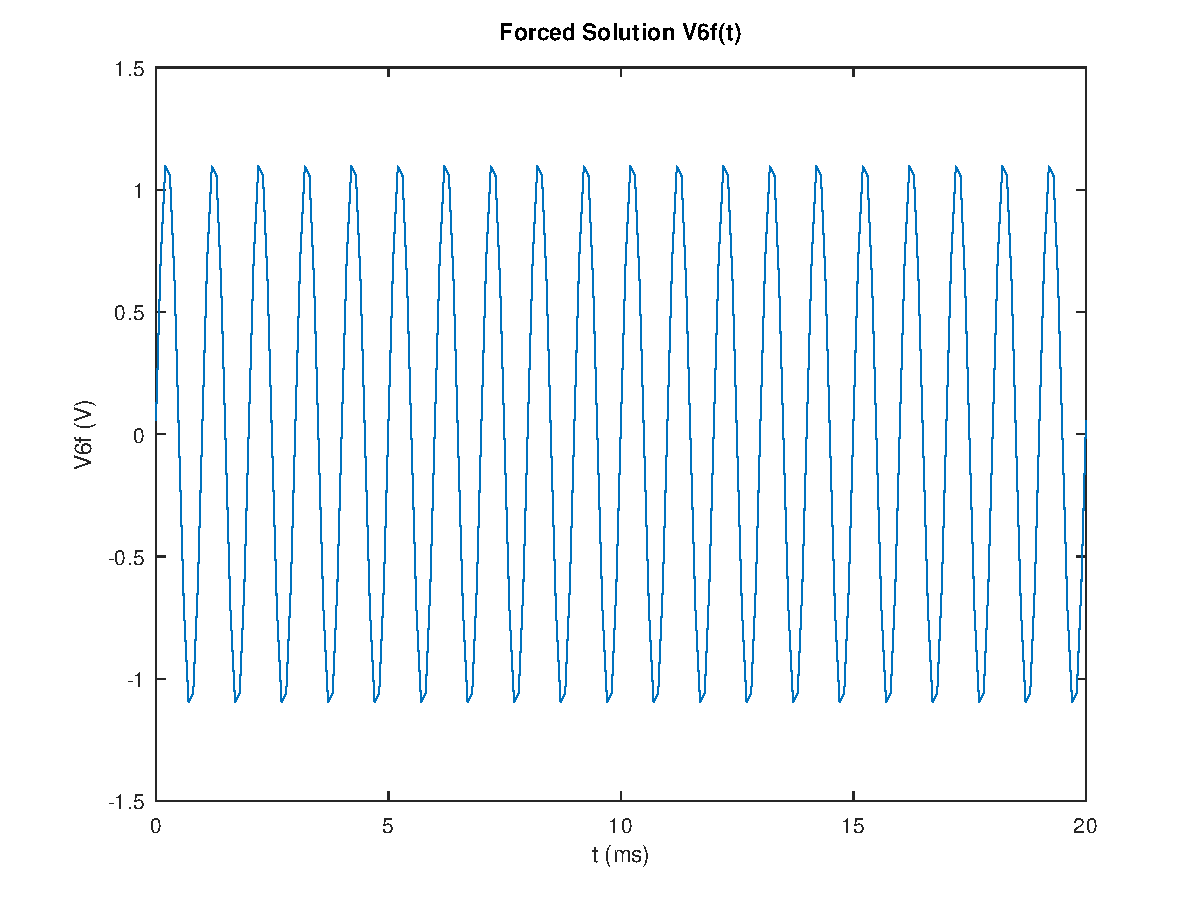
\includegraphics[width=0.7\linewidth]{../mat/alinea4.pdf}
\caption{Plot alinea 4.}
\label{fig:plot4}
\end{figure}


\subsection{Question 5: Final solution $v_{6_t}(t)$ }




